\begin{figure*}[!t]
    \centering
    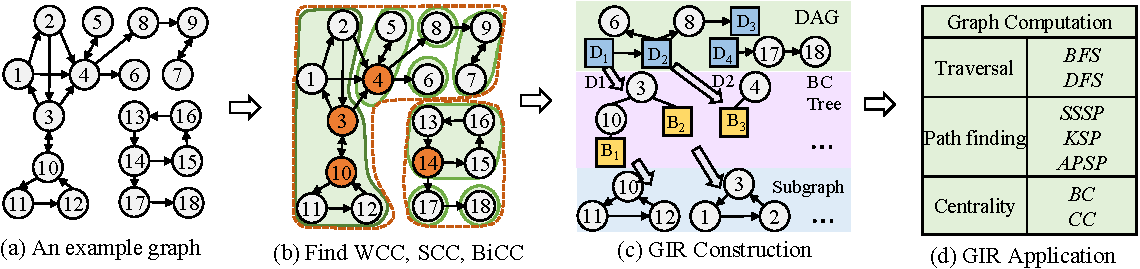
\includegraphics[width=1\linewidth]{figures/gir_framework-crop.pdf}
    \caption{Overview of the pipeline.
    (a) shows an example graph,
    (b) decomposes it into WCCs, SCCs, and BiCCs,
    (c) constructs the GIR,
    and (d) performs downstream graph query analytics on GIR.}
    \Description{Four-panel pipeline diagram: an example graph, its decomposition into WCCs/SCCs/BiCCs, the resulting GIR structure, and downstream query analytics running on GIR.}
    \label{fig:gir}
\end{figure*}

\section{Overview}
\label{sec:methodology}

% \YJ{working on.}

Figure~\ref{fig:gir} overviews the end-to-end pipeline of our method on an exmaple graph.
Particularly, 
GIR operates in three phases: GIR construction, structure-aware incremental maintenance, and GIR-enabled task parallel execution.

% GIR operates in three phases: GIR construction (Section~\ref{sec: construction}), structure-aware incremental maintenance (Section~\ref{sec: maintenance}), and GIR-enabled task parallel execution (Section~\ref{sec:task_parallel}).
% These correspond to the three technical sections that follow
% (Sections~\ref{sec:gir}, \ref{sec:maintenance}, and~\ref{sec:framework}).

% Figure~\ref{fig:gir} presents the overall workflow of \name{} using a directed graph example, covering three components: GIR construction, dynamic maintenance, and GIR-guided analytics.

% GIR is a dynamic, query-agnostic structural index that decomposes a directed graph into three nested layers, as illustrated in Figure~\ref{fig:gir}. 
\textit{(i)} For GIR construction, at the coarsest level, WCCs partition the graph into independent regions. Within each WCC, SCCs are contracted into a condensation DAG, eliminating redundant exploration of cyclic subgraphs, as shown in Figure~\ref{fig:gir}(b). Within each SCC, BiCCs and their block-cut tree expose articulation boundaries, as shown in Figure~\ref{fig:gir}(c). They enable independent processing of structurally isolated subgraphs. Together, these three layers make structural boundaries explicit and directly accessible, replacing boundaries that would otherwise be rediscovered implicitly at query time.

\textit{(ii)} To keep GIR consistent under dynamic updates, we classify every edge insertion or deletion into one of five structurally distinct cases using only pre-maintained metadata. This confines each repair to the minimum necessary region via a scope-prune-update (SPU) strategy for single-edge updates and a filter-merge-update (FMU) strategy for batches.


\textit{(iii)} GIR further unlocks task parallelism as a complement to conventional data parallelism. Because GIR decomposes the graph into independent structural units, multiple units can be processed as concurrent tasks without inter-task synchronization, offering a second dimension of parallelism that flat adjacency representations cannot provide.


% \textbf{GIR construction.} Given a directed graph, GIR decomposes it into three nested structural
% layers, Figure~\ref{fig:gir}(b)(c).
% At the coarsest level, weakly connected components (WCCs) partition the graph into globally
% independent regions.
% Within each WCC, strongly connected components (SCCs) are identified and contracted into supernodes,
% producing a condensation DAG that captures global directed reachability without cycles.
% Within each SCC, biconnected components (BiCCs) decomposition exposes articulation boundaries
% and organizes blocks into a block-cut (BC) tree.
% Figure~\ref{fig:gir}(c) shows the constructed GIR. A super vertex $D_1$ is described by a BC tree with block nodes $B_1$, $B_2$ and AP vertices 3 and 10, making explicit that any path from vertex~2 to vertex~11 must pass through both APs.
% This three-level hierarchy transforms a flat adjacency structure into
% a representation that makes structural boundaries explicit and
% directly accessible to downstream algorithms.

% % This hierarchy of WCCs, condensation DAG, and BC trees constitutes the \emph{Graph Intermediate Representation} (GIR), which materializes structural invariants once for reuse across updates and queries.

% % Given the dynamic directed graph in Figure~\ref{fig:gir}(a), \name{} first builds GIR by decomposing it into three nested structural layers.
% % At the coarsest level, the graph is partitioned into weakly connected components (WCCs).
% % Within each WCC, strongly connected components (SCCs) are identified and contracted into supernodes, producing a condensation DAG that compactly captures global inter-component reachability, as shown in Figure~\ref{fig:gir}(b).
% % At the finest level, each SCC is further decomposed into biconnected components (BiCCs) and organized as a BC tree, where block nodes correspond to BiCCs and articulation nodes correspond to articulation points (APs).

% \textbf{Structure-aware incremental maintenance.}
% When the graph evolves, GIR updates its structural layers
% incrementally rather than recomputing them from scratch.
% \textit{The key insight is that most edge insertions and deletions affect
% only a small local region of the hierarchy}.
% For each update, the designed \emph{scope-prune-update} strategy
% determines which layer is affected, restricts the repair to the
% smallest affected subregion, and performs localized structural fixes.
% For batches of updates, the designed \emph{filter-merge-update} 
% pipeline removes redundant operations and processes
% structurally related updates concurrently.


% % When the graph evolves, \name{} updates GIR incrementally rather than recomputing from scratch.
% % For each edge insertion or deletion, a \textit{scope-prune-update} (SPU) strategy first identifies which GIR layers are affected using lightweight metadata (e.g., DAG ranks), restricts repair to the smallest affected subregion, and then performs localized structural updates.
% % For batch updates, a \textit{filter-merge-update} (FMU) pipeline removes redundant operations and processes structurally related updates concurrently.

% \textbf{GIR-enabled two-level parallel execution.}
% Once GIR is updated, downstream algorithms exploit the hierarchy
% to eliminate redundant work and expose task parallelism
% (Figure~\ref{fig:gir}(d)).
% Given a source query, GIR first prunes unreachable SCCs via the
% condensation DAG.
% It then decomposes the retained region into independent BC-tree
% blocks, each of which becomes an independent task that can further improve the parallelism by enabling task parallelism.
% In the running example, five BFS tasks execute concurrently, a level of task parallelism that flat-graph traversal cannot expose.
% The same decomposition applies to other algorithms, such as SSSP, DFS, and betweenness centrality.



% Once GIR is maintained, downstream analytics exploit its hierarchy for scalable execution, as shown in Figure~\ref{fig:gir}(d).
% Given a query, \name{} prunes unreachable SCCs via the condensation DAG, decomposes the retained region into independent BC-tree blocks for concurrent task execution, and merges local results into a globally consistent output.
% In the running example, five BFS tasks execute concurrently, a level of task parallelism that flat-graph traversal cannot expose.
% The same strategy generalizes to SSSP and betweenness centrality (BC).

% \YJ{Too short. \CQ{done}}


%
%\YJ{TODO: Add the lemmas}

%\textbf{Lemma 1.}  
%Given a directed graph, after decomposing it into SCCs, all BiCCs are contained within individual SCCs.
%\textbf{Lemma 2.}  
%When an insertion occurs in the DAG layer, only nodes whose topological order lies between the affected high-level and low-level nodes may be impacted.

%\textbf{Lemma 3.}  
%During cycle detection or path verification in DAG updates, the search space can be pruned to nodes whose topological ranks lie betw  een the source and target levels.

\section{A Novel Hierarchical Graph IR}

\label{sec: construction}

% We propose GIR as a novel structural layer for dynamic graphs.
% Traditional dynamic graph systems operate directly on adjacency
% structures.
% Each downstream algorithm must repeatedly rediscover connectivity
% boundaries, articulation structure, and reachable regions from
% scratch.
% GIR instead materializes these structural properties once and
% keeps them up to date as the graph evolves.
% Downstream algorithms reuse this maintained structure rather than
% recomputing it.
% This makes GIR query-agnostic: the same structural layer serves different graph algorithms
% without any query-specific precomputation.

% \subsection{Three-Level Structural Hierarchy}
% \label{subsec:hierarchy}

GIR is built on a simple but powerful principle: \emph{separate structural organization from algorithm execution}.
However, not every structural property of a graph deserves to be maintained incrementally.
Instead, we select 
% GIR selects 
invariants that satisfy three criteria simultaneously.
First, the invariant must be \emph{incrementally maintainable}: a single
vertex/edge insertion or deletion must confine repair to the structurally
affected region, not the entire graph.
For WCC and BiCC, this region is provably local (a single component or block).
For SCC, a single edge can in principle merge many SCCs if it closes a large
cycle; however, GIR's rank-based pruning (Section~\ref{sec: maintenance})
bounds the search to the rank interval between the two endpoints, limiting the
work to the actually affected SCCs rather than triggering a global recomputation.
Second, it must be \emph{algorithm-independent}, meaning that it must reflect the structure of the graph itself, not the parameters of any
specific query.
Third, it must be \emph{directly actionable}. That is, a downstream
algorithm must be able to use it to skip work, not merely consult
it as reference.

We observe that connectivity decomposition algorithms, including WCC, SCC (along with condensation DAG), and the BC tree, 
% are 
% three standard connectivity decompositions of a directed graph that
satisfy all three criteria.
Together, they form a complete global-to-local hierarchy with no
gap and no redundancy between levels.
Motivated by this, we design the GIR as a three-level structural hierarchical layer.
% Figure~\ref{fig:gir} illustrates this hierarchy on an example graph.

\textbf{Level 1: WCC}
is chosen as it provides the strongest possible pruning
at zero traversal cost.
No path of any kind can cross a WCC boundary.
A query at any vertex is therefore entirely confined to that
vertex's WCC.
All other WCCs can be eliminated before a single edge is examined.
WCC also has the simplest incremental maintenance rule of the three. That is, one insertion can only merge two WCCs, and one deletion can only split one.
This makes the WCC layer a nearly free filter that benefits every
source-rooted algorithm on the graph.

\textbf{Level 2: SCC}
is used because it resolves the fundamental difficulty of
directed traversal, i.e., cycles.
In a directed graph, any strongly connected region is internally
equivalent for reachability purposes.
Every vertex in an SCC can reach every other vertex in the same
SCC, so the SCC as a whole can be treated as a single unit.
Contracting each SCC into a supernode and connecting them by the
remaining inter-SCC edges produces the condensation directed acyclic graph (DAG).
% which is acyclic by construction.
This transforms directed reachability into a DAG walk, eliminating
all cycle-related redundancy.
The DAG also yields a topological order that lets algorithms
process SCCs level by level without backtracking.
Incrementally, one edge insertion can at most merge SCCs by creating
a new directed cycle, and one deletion can at most split one SCC.
Both operations are local and do not affect the rest of the DAG.

\textbf{Level 3: Block-cut tree}
is selected as it exposes the finest level of independent
substructure within an SCC.
Even inside a strongly connected region, the internal topology is
not uniform.
Some vertices are articulation points (APs), whose removal will disconnect
the SCC into separate regions.
Any path between vertices in different BiCC blocks must pass through these APs.
This property holds unconditionally, regardless of algorithm type.
Therefore, we can exploit it to decompose execution. That is, each BiCC block can be
processed as an independent task, enabling task parallelism
across blocks without inter-task synchronization.
The BC tree organizes blocks and APs hierarchically, exposing the entry point of each block and making the task decomposition explicit.
% Incrementally, a single edge update typically affects only the
% block containing that edge.
% The BC tree repair is therefore confined to a small local region
% even within a large SCC.


% An algorithm that uses all three levels first discards irrelevant
% components, then navigates a cycle-free inter-SCC structure,
% then executes concurrently within independent blocks.



% Section~\ref{sec:maintenance} describes how GIR is maintained
% incrementally under continuous updates.
% Section~\ref{sec:framework} describes how downstream algorithms
% exploit the hierarchy for parallel and efficient computation.

% \subsection{Scope of Benefit}
% GIR is most beneficial for algorithms whose execution can be pruned, decomposed, or reordered using structural boundaries. 
% The three GIR levels provide three types of structural knowledge that enable three corresponding optimizations.

% \textit{WCC (Level 1) is for scope elimination}. Any single-source algorithm on a directed or undirected graph can immediately discard all WCCs that do not contain the source. This benefits many algorithms, such as, BFS, DFS, SSSP, APSP (per-source), reachability queries, betweenness centrality (which issues SSSP from every vertex), $k$-shortest paths. Essentially any algorithm that starts from a specific source benefits.

% \textit{Condensation DAG (Level 2) is for cycle elimination.} On a directed graph, any algorithms that must follow directed paths can use the DAG to prune reachable SCCs before walking raw edges. This benefits algorithms, such as SSSP, directed reachability, topological-order-dependent algorithms, and dependency-chain analysis. Algorithms that need to traverse only forward-reachable SCCs can skip cycles entirely.

% \textit{BC tree (Level 3) is for task decomposition}. Any algorithms that can process subgraphs independently and then merge results benefits. This is the basis of GIR's task parallelism contribution. BFS, DFS, SSSP, and betweenness centrality all have this property. The BC tree also enables localized updates, i.e., when GIR is maintained after an edge change, only the affected BiCC block needs to be repaired.

% % GIR is most beneficial for algorithms that issue queries from
% % a specific source or target, or that traverse directed paths.
% % This class includes BFS, DFS, SSSP, all-pairs shortest paths
% % (via per-source SSSP), betweenness centrality, closeness
% % centrality, reachability queries, and k-shortest paths.
% % For these algorithms, GIR enables two distinct optimizations.
% % First, WCC and DAG structure prune the search space before
% % traversal begins.
% % Second, BC-tree decomposition exposes task parallelism across
% % independent BiCC blocks.

% Algorithms that aggregate globally across all vertices, such
% as PageRank~\cite{page1999pagerank} and label propagation~\cite{zhu2002learning}, might not directly benefit from the
% condensation DAG or BC tree.
% They operate on all edges regardless of source, so
% structural boundaries do not reduce their work.
% However, these algorithms still benefit from WCC-level
% partitioning. That is, separating WCCs can be processed independently
% and in parallel.
% After that, the updates confined to one WCC require
% only that component's scores to be updated.
% We would not claim of benefit for global aggregation algorithms beyond this.

%\textbf{GIR design.}
% We propose GIR as a hierarchical graph intermediate representation built upon three fundamental decompositions: weakly connected components (WCCs), strongly connected components (SCCs), and biconnected components (BiCCs)~\cite{tarjan1972depth, tarjanscc1972depth, hopcroft1973algorithm,ji2018ispan,ji2020aquila}.
% As illustrated in Section~\ref{sec:methodology}, these form three nested structural layers---WCCs, the SCC condensation DAG, and per-SCC BC trees---that together make connectivity structure explicit and reusable.
% Here we focus on three design aspects that are not covered in the overview: structural--execution separation, storage compatibility, and extensibility.


% \subsection{old}
% A key feature of GIR is that it separates \emph{structural organization} from \emph{algorithm execution}.
% Traditional dynamic graph processing often operates directly on adjacency structures, forcing each downstream task to repeatedly rediscover connectivity boundaries, critical connectors, and affected regions.
% In contrast, GIR materializes these structural invariants once and reuses them across multiple tasks.
% For example, the condensation DAG can be used to prune unreachable SCCs during traversal or path computation, while the BC tree can localize exploration to only those BiCCs and articulation boundaries that are relevant to a given query.
% This makes GIR query-agnostic: the same structural representation can support many different downstream computations, such as reachability, traversal, and path finding~\cite{tarjan1972depth,gross2005graph,nagamochi2000graph}, without requiring each algorithm to rebuild structural knowledge from scratch.

% Another important aspect of GIR is that its hierarchy naturally supports scalable execution.
% The WCC, SCC, and BiCC layers form explicit structural partitions that can be used as independent or semi-independent computation units.
% At the global level, different WCCs can often be processed separately.
% Within a WCC, SCC supernodes provide a compact execution scope for many graph tasks.
% Within an SCC, BiCCs and articulation points further expose localized substructures that can be processed selectively.
% This hierarchical decomposition is particularly suitable for multi-threaded and GPU systems, where component-level parallelism and localized memory access are critical for performance.
% Our previous systems, Aquila~\cite{ji2020aquila} and iSpan~\cite{ji2018ispan,ji2022ispan}, already demonstrate that WCC, SCC, and BiCC decompositions can be computed at high throughput on billion-edge graphs, which makes GIR a practical foundation for large-scale dynamic graph analytics.

% GIR is also designed to work with dynamic graph storage rather than replacing it.
% The representation can be integrated with existing dynamic graph formats such as PMA~\cite{bender2007adaptive}, DCSR~\cite{king2016dynamic}, Terrace~\cite{pandey2021terrace}, and DGAP~\cite{islam2023dgap}.
% In this sense, GIR serves as a structural layer above the underlying storage layer: the storage format is responsible for maintaining graph data efficiently under updates, while GIR is responsible for exposing reusable structural invariants for analytics and maintenance.
% This separation improves modularity and allows GIR to be incorporated into existing dynamic graph systems without redesigning the entire storage stack.

% Although the current instantiation of GIR focuses on WCC, SCC, and BiCC, the framework itself is intentionally extensible.
% These three decompositions are the core structural primitives in our current design because they provide a strong balance between expressiveness, computability, and practical usefulness.
% However, the abstraction is not limited to them.
% Additional structural indices or auxiliary representations, such as dominator trees or reachability indices, can be incorporated whenever they provide value for dynamic maintenance or downstream analytics.
% This makes GIR a general structural framework for dynamic graph systems rather than a fixed-purpose representation.

% Overall, GIR transforms a flat dynamic graph into a layered structural representation that explicitly captures both global connectivity and local articulation structure.
% By organizing the graph into reusable WCC, SCC, and BC tree layers, GIR provides a common framework for structural maintenance, query pruning, and scalable downstream computation.
% This hierarchical design is the key that allows GIR to support efficient updates while also accelerating diverse graph analytics.

% \YJ{Example}
% In Figure~\ref{fig:pre_process}, nodes prefixed with `a' denote APs, and nodes prefixed with `b' denote BiCCs. There are two important properties of the BC tree that lay the foundation for us to exploit it to KSP computation:
% These BiCCs serve as logical submodules that support efficient localized computation and resilience analysis. The BC tree structure not only enables rapid evaluation of queries like fault impact or neighborhood exploration, but also allows future integration of fine-grained update strategies on a per-block basis.
% \YJ{Explain our BC+ tree idea.}
% \YJ{Can add the lemma of AP in SCC here.}


